\iffalse
https://edoc.sub.uni-hamburg.de/hcu/volltexte/2017/370/pdf/Ebert_Kirsten.pdf Anfang
\fi
%synonym handelsmodelle

\begin{folding} % Einleitung

Im folgendem werde ich Vertriebe aller Art ähnlich wie im Buch "Das E-Commerce Buch: Marktanalysen - Geschäftsmodelle - Strategien" unterteilen: in Online-Marktplätze sowie -Händler, Kataloversender, stationäre Händler, Hersteller und Unternehmen der Diensleistungsbranche\cite[S. 15ff]{Graf}. Dabei sind Online-Marktplätze eine Art Online-Vermittler zwischen Kunden und Verkäufer, Online-Händler bieten dagegen nur eigene, meist sehr spezialisierten Sortimente an. Kataloversender verhalten sich ähnlich: sie versenden ihr Sortiment direkt an Kunden. Stationäre Händler verkaufen im Gegensatz zu den genannten Vertreibsstrukturen in Fillialen und sind mit Kataloghändlern am stärksten von den Änderungen der letzten Jahrzenten betroffen. Während sich die genannten Unternehmensarten meistens am Ende der Verkaufskette befinden, stehen Hersteller am Anfang: sie stellen Güter her und sind dementsprechend, insofern sie nicht selber den Verkaufsprozess übernehmen, auf weitere Unternehmen für Verkauf und Vermarktung angewiesen(ebd.). %vor und -nachteile?; beispielsunternehmen

\end{folding}

\begin{folding} \subsubsection{Kataloghändler}

Kataloghändler sind die größten Verlierer der letzten Jahrzehnte: mit der Entwicklung des Onlinehandels ist ab 2002 schon ein Rückgang der Nachfrage zu spüren – einige eröffnen eigene Online-Shops\cite[S. 24f]{Graf}, jedoch oft mit wenig Erfolg\cite[S. 38]{Graf}. 2015 sind Katalogversender fast ausschließlich verschwunden oder zu Online- und Einzelhandel konvertiert, da sie kaum einen Mehrwert im Vergleich zum klassisschen Onlinehandel bieten\cite[S. 47]{Graf}. So prognostiziert beispielsweise 2012 IFH Retail Consultants einen einen sinkenden Anteil des Online-Umsatzes von 24.9\% zu 23.9\% in den folgenden 2 Jahren\cite[S. 20]{evilcom}. Tatsächlich fiel der Anteil aber ganze 3.6\% - knapp das vierfache des erwarteten Wertes. In den Folgejahren verhielt sich der Rückgang der Katalogdrucke linear und betrug von 2011 zu 2019 "nur" 17.2\%.\cite{statista-katalog}. Aufgrund der fehlenden Relevanz der Kataloghändler - insbesondere mit Blick auf die Zukunft - werde ich sie im Rahmen dieser Arbeit nicht weiter berücksichtigen. 

\end{folding}

\begin{folding} \subsubsection{Stationäre Händler}
    % nitt S 54 these, dass einzelhandel zurückkommt
Der stationäre Handel ist einer der wichtigsten Vertriebsbestandteile und Dank seiner noch größeren Bedeutung in der Vergangenheit nahezu überall vertreten. Viele stationäre Vertriebe können gleichzeitig als Einzelhandel eingeordnet werden, diese
\begin{quote}
    "[...] die Produkte unterschiedlicher Hersteller zu einem Sortiment zusammenfass[en] [...] und nur an Konsumenten und nicht an gewerbliche Kunden verkauf[en]."\cite[S. 20]{Ebert}
\end{quote}
Jedoch gibt es auch andere, nicht unwichtige, stationäre Unternehmen, die nicht in die Kategorie des Einzelhandel fallen, wie beispielsweise den stationären Teil des Dienstleistungsektors. Im Rahmen dieser Arbeit haben wir mit dem selbstständigen Architekten Prof. Dr.-Ing. André Spindler ein Interview geführt, um Einblicke in diesartige Firmen zu erlangen. Auf diese werde ich später noch detailiert eingehen, jedoch bildet der Einzelhandel den Hauptpunkt dieser Arbeit, da er insbesondere im ländlichen Bereich deutlich stärker vorhanden ist. Zudem ist es möglich, diesen in Betracht des Verkaufsablaufes weiter einzuordnen. Dabei bilden sich vor allem folgende 3 Arten heraus: Einerseits der ambulante Einzelhandel, der an keinen festen Ort gebunden ist und sich selber zu seinen Kunden bewegt, wie z. B. Eiswagen. Diese Art von Einzelhandel stellt mittlerweile in Deutschland einen sehr geringen Teil dar und wird im Rahmen dieser Arbeit nicht berücksichtigt. Ein weiter Vertriebskanal bildet der Distanthandel, der hierbei größtenteils mit unter den Punkt Onlinehändler- und Marktplätze, jedoch auch z. T. unter Kataloghändler fällt. Die letzte Art ist der stationäre Einzelhandel, der im folgenden charakterisiert wird(ebd.).

Der stationäre Handel ist durch die steigende Relevanz des Onlinehandels weniger gefragt denn je und versucht mit strukturellen Änderungen dagegen anzukämpfen. Einige Einzelhändler eröffenen paralel zu ihrem Geschäft einen Online-Shop, andere bieten die Möglichkeit, Waren online in den Laden zu bestellen und diese dort anzuholen – sogenanntes "Multichannel-Marketing", das Ansprechen der Kunden über mehrere Vertiebswege\cite[S. 34f]{Graf}. Jedoch fahren die neuen Strkturen nur wenig Erfolge ein – so erhöhen sie zwar die Onlinepräsenz, bieten jedoch nur einen geringen Mehrwert im Vergleich zu den bekannten Onlineriesen wie Amazon\cite[S. 34f]{Graf}. 

Heute hat der lokale Handel einige schwerwiegende Probleme: 
Beispielsweise ist der stationäre Aspekt besonders im ländlichen Raum eher ein Hindernis: So weichen viele Familien beim Einkaufen auf Städte in der Umgebung aus. Diese Problematik hat sich in unserer Schülerumfrage am hennebergischen Gymnasium "Georg Ernst" bestätigt: 68.7\% der 147 Befragten gaben an, regelmäßig außerhalb Schleusigens einzukaufen - meistens nach Suhl oder Coburg. 
Auch die geringe Auswahl sowie schlechte Jugendorientierung erwähnten viele Teilnehmer als Schwäche des lokalen Handels(siehe Anhang). Schließlich stellt sich die Frage, welche Vorteile der stationäre Handel noch bieten kann, um die im Vergleich zum Onlinehandel deutlich höheren Preise zu rechtfertigen - denn pure Onlinehändler haben deutlich dünnere Kostenstrukturen\cite[S. 14]{evilcom}. So müssen sie etwa keine Miete für Geschäfte zahlen und kommen mit deutlich weniger Angestellten aus, folglich weniger Kosten. 

Einer dieser Vorteile ist in der Theorie der soziale Aspekt des Einkaufens, der laut Nitt-Drießelmann vorallem für über-50-Jährige, die über viel Freizeit verfügen, eine immer größer werdende Rolle spielen wird\cite[S. 43f]{Nitt}:
\begin{quote}
"Als Mittel gegen Vereinsamung und Anonymisierung im Alltag wird die soziale Komponente beim Einkaufen [...] zunehmend an Bedeutung gewinnen."\cite[S. 43]{Nitt}
\end{quote} 
So soll in Zukunft der Wunsch nach Begegnungen mit bekannten Personen und Beratung zunehmen und die Zusammensetzung von sozialen Kontakten auch bei der Wahl des Vertriebsweges eine immer wichtigere Rolle spielen(ebd.).
Außerdem müssen stationäre Einzelhändler stärker auf die geänderten Wünsche von Konsumenten eingehen. Beispielsweise legen viele Konsumenten eine broßen Wert auf einen bequemen Einkauf mit langen Öffnungszeiten, eine übersichtliche Warenpräsentation sowie eine möglichst große Produktauswahl auf einer so kleinen Verkaufsfläche wie möglich\cite[S. 61]{Nitt}.

Zu dem kommt, dass in Deutschland bedeutende demografische Änderungen bevorstehen: so schrumpft und altert die Gesamtbevölkerung, folglich müssen alle Bereiche des stationären Handels sich auf einen zusätzlichen Nachfragerückgang einstellen sowie die Bedürfnisse von Senioren stärker beachten - insbesondere auf dem Land, denn in Metropolen soll das Durchschnittsalter nahezu konstant bleiben\cite[S. 32ff]{Nitt}. Im Rahmen dieser Erkenntnis ist es für den Offlinehandel wichtig, mehr auf die Bedürfnisse der älteren Bevölkerungsschicht, die 2050 etwa 59\% der Kaufkraft ausmachen soll, einzugehen\cite[S. 64]{Nitt}. So kaufen Sie oft qualitativ hochwertigere in den Bereichen Gesundheit, Wohnen und Energie - jedoch eher selten langlebige Konsumgüter, da Sie diese schon besitzen; zusätzlich sehen sie kein Problem damit, für kompetente Beratung mehr zu bezahlen\cite[S. 41f]{Nitt}. Folglich muss der stationäre Handel die Produktauswahl sowie Erreichbarkeit und Übersichtlichkeit auf die alternde Bevölkerung anpassen, um die beste Kaufoption für Sie zu bleiben\cite[S. 64]{Nitt}.

Obwohl in Zukunft die Bevölkerung Deutschlands schrumpfen wird, ist eine erhöhte Anzahl von Haushalten zu erwarten - durch eine "Zerstreuung" der Haushaltsstruktur. So soll es 2030 1.8 Mio. weniger Mehrpersonenhaushalte geben, dafür aber 1.4 Mio. Einpersonen- sowie 1.6 Mio. Zweipersonenhaushalte mehr als 2010\cite[S. 35]{Nitt}, was zu einer automatischen Erhöhung der Wochnfläche pro Person führt. So werden Haushaltsprodukt- und Möbelverkäufer in den nächsten Jahren weniger von Insolvenzen betroffen sein wie Unternehmen anderer Branchen.

Ein weiterer Vorteil des stationären Handels sind Produkte, die nicht oder nur schwer durch andere Vertriebswege abzudecken sind, wie etwa beratungsintensive Waren. Auch die Möglichkeit, Produkte direkt zu Testen und die sofortige Verfügbarkeit sorgt für Umsätze des analogen Handels\cite[S. 2]{Maier}. Außerdem trugen im stationären Handel
\begin{quote}
 "sogenannte \ac{FMCG}, also schnelllebige Verbrauchsgüter wie   Drogerieartikel,   Tiernahrung   oder   Lebensmittel,   mit 42,5 Prozent mit Abstand den größten Teil zum Gesamtumsatz 2018 bei"\cite{corona-schub}.
\end{quote}

\noindent Im Rahmen unserer Online-Umfrage von Schülern des hennebergischen Gymnasium "Georg Ernst" konnten wir dies  bestätigen:  
 \begin{figure}[h]
    \begin{center}
        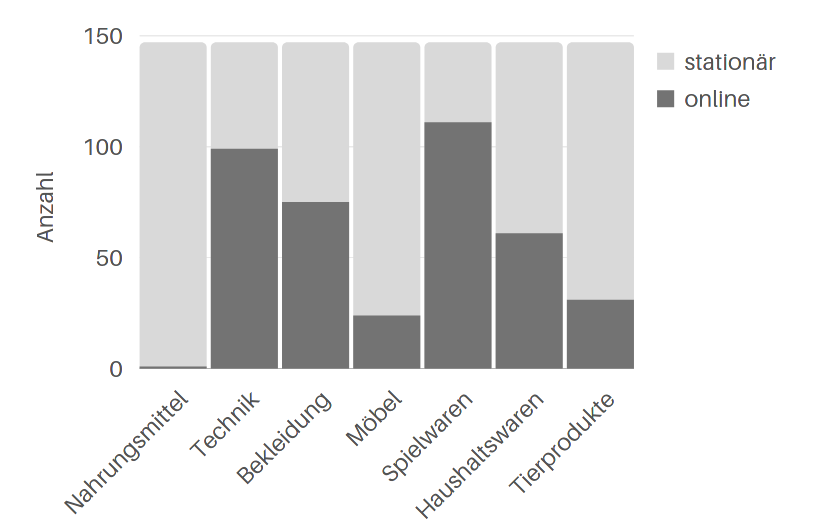
\includegraphics[width=8cm]{media/schuelerumfrage/1.png}
        \caption{Bevorzugter Kaufweg nach Produktgruppe}
        \label{Kaufwege}
        \bildquelle  eigene Darstellung
    \end{center}
\end{figure}
so werden insbesondere Nahrungsmittel nahezu ausschließlich stationär gekauft. Andere Güter, die nicht in die Produktgruppe der \ac{FMCG} fallen, werden dagegen oft auch online gekauft. Wenn man den stationären Nachfragerückgang durch den Distanzhandel betrachtet, kann man die \ac{FMCG} als "verlässliche Umsatzlieferanten" einordnen. - Sie helfen, Verkäufe kurzfristig konstant zu halten sowie langfristig den Online-Einfluss abzudämpfen. Jedoch wird durch die Corona-Krise die Nachfrage nach flexiblen und bequem zugänglichen Produkten erhöht - auch im Produktbereich der \ac{FMCG}(ebd.). Eine ausführliche Diskussion dieser Thematik findet sich in Kapitel [4.4.2].

%https://de.statista.com/statistik/daten/studie/201914/umfrage/einkaufsverhalten-im-onlinehandel-vs-einzelhandel-nach-produktgruppen/

%handwerker: kaum durch online ersetzbar, allerdings ist ein pur stationärer handwerkerbetrieb auch nicht zukunftsfähig.
\end{folding}

\begin{folding} \subsubsection{Dienstleistungsektor am Beispiel der Architekturbranche}

Neben dem Einzelhandel sind auch andere stationäre Firmen vom Wachstum des Onlinehandels betroffen. Wie bereits angesprochen konnten wir Dank unserem Interview mit Prof. Dr.-Ing. André Spindler einige Unterschiede in der Online-bedingten Entwicklung des Dienstleistungsektors im Vergleich zum Einzelhandel feststellen.

Zuerst ist anzumerken, dass der stationäre Handel eine sehr variable Struktur besitzt und sich dementsprechend die Entwicklungen der letzten Jahrzehnte auf verschiedene Teilbereiche sehr unterschiedlich ausgewirkt haben. So ist beispielsweise das Einbinden der Onlinepräsentation durch Websiten o. ä. in der Architekturbranche

\begin{quote}
"[...] eigentlich seit Anfang an üblich – also seit dem es dieses Medium gibt, weil die Architekten natürlich im besonderen Maße visuell werben [...]."(Spindler, André, persönliches Interview, Erfurt, 19. 09. 2020, siehe Anhang [], 00:04:12)
\end{quote} 
Prof. Spindler verweist dabei zusätzlich darauf, dass es für den Großteil der Architekturbranche schwierig ist, allein mit Werbung durch Printmedien zu überleben und deshalb eine Online-Präsenz vonnöten ist(ebd.), jedoch treffen diese Annahmen nicht auf seine Brandschutz-Nische zu, da diese in die Kategorie "Verkauf von Wissen" fällt, auf welche man das Konzept des Onlinehandels nicht ohne Probleme anwenden kann(siehe Anhang [], 00:11:05). Prof. Spindler beschrieb die Problematik folgendermaßen:

\begin{quote}
"[...] wir werben ja nicht mit einer schönen Fassade wie der Architekt, sondern wir werben mit einer Fachplanung, die man möglichst gar nicht sehen soll, sondern die dann wirkt, wenn es brennt und die vorher gar nicht in Erscheinung treten soll. Wir machen natürlich viel mehr in Konzeption, die sich nicht so leicht visualisieren lassen."(siehe Anhang [], 00:06:37)
\end{quote} 

Zusäzlich lässt sich auf viele Vertriebe, wie auch das Unternehmen Spindlers, das Prinzip des klassischen Handels nicht anwenden. 

\begin{quote}
"[...] dass man sagt, da gibt's ein Angebot und das nehme ich jetzt als Kunde an. Sowas geht bei uns nicht. Und zwar nicht nur bei uns nicht, sondern ich glaube, in der ganzen Branche macht man das nicht, weil wir ja nicht ein einzelnes Produkt [...] anbieten, verkaufen, sondern eine recht komplexe Tätigkeit. Und wir brauchen, um überhaupt einen Preis zu finden, dem man dann annehmen könnte eine ganze Reihe Informationen. [...] Deswegen, denke ich, wird es in vielen Dingen so sein, dass man erst einmal in den Austausch geraten muss."(siehe Anhang [], 00:06:37)
\end{quote} 
Aufgrund von Problemen wie diesem blieb der Dienstleistungsektor, welcher einen nicht unrelevanten Teil seiner Arbeit ausmacht, noch weitesgehend unbeeinflusst von der Vernetzung seit der Jahrtausendewende. Durch die schwierige Präsentation, Vermarktung sowie Verkauf in Prof. Spindlers Fachgebiet spielt der Online-Aspekt für ihn eine weniger relevante Rolle. Trotzdem steigt die Nutzungszahl von Online-Elementen, wenn auch in diesem Fall etwas träge, ständig. So gibt es beispielsweise Pilot-Landkreise, die Vorgäge vollständig digital bearbeten - Sie hatten Anfangs Probleme, können trotzdem aber eine positive Zwischenbillaz ziehen(Anhang [], 00:20:35). Zudem ist das Vermeiden von planungsbedingen Problemen durch sogenannte \ac{BIM}-Systeme, die elektronisch eine konfliktlose Planung ermöglichen(Anhang [], 00:31:22). Trotzdem sind immer noch viele Fragen bzgl. der elektronischen Datenverwaltung in Unternehmen ungeklärt.

\begin{quote}
"[...] ein Kollege hat mal so aus Spaß gesagt, wir können doch nicht auf dem Bildschirm stempeln. Wie machen wir das dann? Wie machen wir ein solches Dokument als geprüftes Dokument kenntlich? Wie sichern wir diese Prüfung, dass sie niemand fälschen kann?."(siehe Anhang [], 00:17:43)
\end{quote} 
All diese Online-Implementationen der Daten- und Prozessverwaltung werden insbesondere in der Zukunft eine bedeutende Rolle spielen - Arbeit erleichtern, sie effektiver machen - jedoch sind sie noch nicht in allen Bereichen notwendig sogar Stand der Technik.

Auch wenn in seinem Fall noch mehr Kunden analog als digital auf ihn stoßen, gibt es trotzdem einige Online-Elemente, die in seiner Tätigkeit eine wichtige Rolle spielen. Auf die Frage, welche Rolle seine Website \emph{dr-spindler.de} im Konsumverlauf spiele, antwortete er, dass zwar vereinzelt Personen über sie auf ihn stoßen, jedoch hat sie viel mehr eine Informationsfunktion: So wird über sie sein Team kurz vorgestellt, Unterlagen wie Nachweise oder Formblätter öffentlich zur Verfügung gestellt sowie Fragen beantwortet(Anhang [], 00:11:05). Prof. Spindler sowie die Baustellen, zu denen er Kontakt hatte, bewerteten diese Entwicklung in erster Linie als positiv, jedoch stellten sie einen bedeutenden Nachteil fest: das Fehlen von direkter, menschlicher Interaktion. 

\end{folding}

\begin{folding} \subsubsection{Onlinehändler und -marktplätze}

Die Onlinehändler und -marktplätze sind die Gewinner der letzten 20 Jahre – die Verkäufswerte wuchsen ab der Jahrtausendwende konstant an und stellen in vielen Branchen für andere Vertriebsstrukturen eine ernst zu nehmende Konkurrenz dar\cite{wolf}. Vorerst wechseln Konsumenten von Katalogen, ab 2010 auch viele Nutzer anderer Verkaufswege, da das Kaufen online fast immer einen Preisvorteil bietet\cite[S. 31]{Graf}.
\begin{figure}[h]
    \begin{center}
        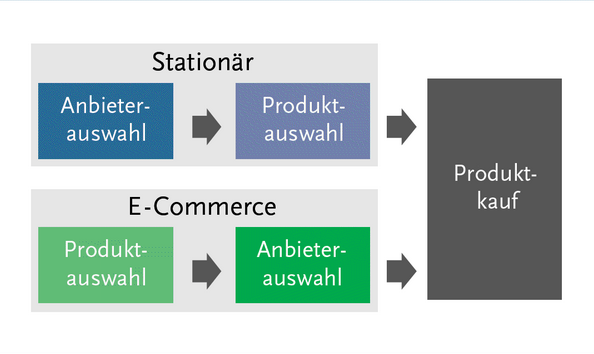
\includegraphics[width=8cm]{media/Fabian-konsumwandel.png}
        \caption{Kaufprozess im Vergleich – Stationär und E-Commerce}
        \label{konsumwandel}
        \bildquelle Björn Schäfers: Social Shopping für Mode, Wohnen und Lifestyle am Beipiel Smatch.com. In: Web-Exzellenz im E-Commerce, Gabler, S. 313 %lieber quelle e com buch???
    \end{center}
\end{figure} 
Außerdem hat sich unter Nutzern des Onlinehandels ein neues Konsumverhalten entwickelt. Bis dahin wa es üblich, zuerst den Anbieter, danach das zu kaufende Produkt auszuwählen; jedoch hat der ab der Jahrtausendewende immer bekannter werdende Onlinehandel dieses Verhalten invertiert\footnote{umkehren}, da das Vergleichen mehrerer Produkte im Internet um ein vielfaches einfacher ist als stationär, allein schon aufgrund des Zeitaufwands für das Besuchen von mehrern Geschäften\cite[S 22f]{Graf}. Auch die Beratung des stationären Handels spielt hier eine Rolle: Online-Käufer informieren sich oft selber und können auf Basis ihrer Recherche das optimale Produkt wählen, während beim Kauf vor Ort meist auf einen bestimmten Verkäufer und dessen Beratung vertraut wird\cite[S. 15f]{evilcom}. Infolge dessen sind Verbraucher, die bereits einmal online eingekauft haben, oft sehr preissensibel - und das auch bei Käufen vor Ort\cite[S. 60]{Nitt}. Aufgrund dessen beschweren sich immer mehr Einzelhändler über den sogenannten "Showrooming-Effekt", das Kaufen von Produkten online, nachdem Beratung eines stationären Händlers in Anspruch genommen wurde. Das dieser Effekt aber auch umgekehrt vorhanden ist, wird meist nicht angesprochen\cite[S. 21f]{evilcom}.
Neu unter Konsumenten ist auch das Bedürfnis nach individiuellen und auf den Käufer angepassten Produkten\cite[S. 43]{Nitt}, was wahrscheinlich durch die extrem große Außwahl bei dem Online-Shopping hervorgerufen wurde. In diesem Aspekt kann der stationäre Einzelhandel schlicht nicht mithalten, da Raum für Produkte stärker begrenzt und preisintensiv ist.

\end{folding}

\begin{folding} \subsubsection{Hersteller}

Ähnlich wie der stationäre Handel sehen Hersteller den Onlinehandel zuerst in einem negativen Licht - aufgrund von untransparenten Verkäufern und möglichen negativen Imageeffekten\cite[S. 20]{Graf}. Zudem entstehen 2002 erste, sogenannte "Powerseller", die im Großhandel Markenprodukte kaufen und deutlich unterhalb des Einzelhandels-Preisniveaus verkaufen\cite[S. 26]{Graf}. Mit der Zeit bauen Marken jedoch verzögert, aber schneller als der stationäre Handel immer mehr eigene Verkaufsportale, um ihre Güter direkt ohne eine Zwischeninstanz zu verkaufen und steigern ihren Umsatz damit bedeutend – beispielsweise verlässt Hugo Boss 2013 Zalando um Produkte über die eigene Website hugoboss.com zu verkaufen\cite[S. 48f]{Graf}. Außerdem wird durch das direkte Feedback eine bessere Produktentwicklung und Kundensupport ermöglicht\cite[S. 39]{Graf}. So ist der Direktverkauf von Marken erfolgreicher denn je, denn sie bieten im Vergleich zu Online-Marktplätzen neben einer besseren Auswahl auf einem bestimmten Gebiet oft deutlich informativere Produktbeschreibung - sprich, bei Produkten einer Brance werden öfter Anbieter nachgefragt, die sich auf diese spezialisieren\cite[S. 18f]{evilcom}.

Außerdem ist dieser Direktverkauf in fast allen Fällen weniger kostenintensiv als der Vertrieb über zusätzliche Instanzen wie den Einzelhandel. Der Rückgang des stationären Konsums ist demnach auch auf die Zunehmende Implementierung\footnote{Durchführung, Nutzung} von Direktverkaufswegen zurückzuführen. Großhandel, die im Gegensatz zu dem Einzelhandel im klassischen Verkaufsprozess früher vorkommen und ihre Güter ausschließlich an gewerbliche Kunden verkaufen, teilen dieses Schicksal(ebd.).

\end{folding}

\begin{folding} \subsubsection{Konsumverhalten allgemein}

Das Konsumverhalten hat sich auch unabhängig von der Handelsstruktur geändert: statt gleichbleibenden, rationalen Käufen und Kaufmotiven, die die Auswahl der gekauften Güter stark abhängig von der zur Verfügung stehenden Geldmenge machten\cite[S. 38]{Schramm}; herrscht heute ein deutlich dynamischeres Kaufklima:
\begin{quote}
"So beziehen jetzt zum Beispiel auch solvente Kunden ihre Lebensmittel aus dem Billigdiscounter, während  umgekehrt  einkommensschwächere  Schichten  zu  Luxusgütern  greifen."\cite[S. 43]{Nitt}
\end{quote}
Außerdem gibt es kaum noch "pure" Einzelhändler und Onlinehändler – meist sind Firmen in mehreren Bereichen vertreten, um ihre Präsenz zu steigern. So eröffnet etwa Amazon in den letzen Jahren Läden vor Ort und stationäre Händler betreiben Online-Shops\cite[S. 50]{Graf}.
Anzumerken ist auch, dass das Konsumverhalten in Deutschlands seit Jahren durch eine starke Kaufkraft geprägt ist, z. T. dank dem 0\%-igen Leitzins der \ac{EZB}\cite[S. 49]{Ebert} – auch wenn die derzeitige Corona-Situation diese leicht abgeschwächt hat\cite{BfWE}. 

\end{folding}



\iffalse 

        EVILCOM --------------------------------------------------------------
        
        auch ältere kaufen online ein: evilcom S 8
        
        durchschnittlicher warenkorbwert steigt, zeichen für mehr akzeptanz des online-shoppings in deutschland. ec S 9
        
        beratung verliert an bedeutung S17
        
        pro-arbeiter-umsatz: stationär 210000 amazon 710000: weniger arbeiter werden bei gleichem konsumverhalten benötigt. jedoch ist amazon deutlich effektiver als die meisten anderen anbieter. trotzdem könnte amazon den effizienztrend weiter antreiben \s. 27 werden logistikdienste nicht als eigene mitarbeiter bei amazon gezählt: die zahl ist also geringer ``nur mit vorsicht zu genießen''
        
        weniger arbeitsplätze vor allem in der zukunft wegen effizienzsteigerungen \S. 28
        
        
        NITT----------------------------------------------------------------
        
        verkaufsflächen steigen beim einzelhandel https://de.statista.com/statistik/daten/studie/462136/umfrage/verkaufsflaeche-im-einzelhandel-in-deutschland/: ist jedoch nicht mit wachstum gleichzusetzen. bezieht sich auf gesamte fläche, nicht nur auf die teueren innenstadtflächen. demnach ist eine umlagerung zu flächen am stadtrand denkbar.
        
        --> unsatz pro fläche (flächenproduktivität) sank bis auf die letzten jahre konstant. diese änderung könnte bedueten, dass der einzelhandel wieder fuß fassen konnte (steigende mieten?). ist jedoch mit vorsicht zu genießen , denn das verkaufen von wenig genutzten grundstücken führt auch zu einer erhöhung der flächenproduktivität:https://de.statista.com/statistik/daten/studie/214701/umfrage/flaechenproduktivitaet-im-deutschen-einzelhandel/
        denn gesamtumsätze fallen seit 1990 stetig\cite[S. 6]{Nitt}
        
        in vielen bereichen verlagern sich stationäre händler in (größere) städte, weg von Land und Kleinstädten. jedoch gibt es auch branches mit wenig veränderung, zb nahrungsmittel
        
        pendler und angestellte kaufen oft nicht in ihrem heimartort sondern am arbeitsplatz ein S 58
    
    
    
    
    
    
        
        allgemein online: großes wachstum ab 2002 S. 26
            jüngere kaufen mehr online ein S 35f
            kleinere haben wenig chancen, da große wie amazon durch hohes kapital niedrige preise finanzieren können, was einer der wichtigsten faktoren beim onlinehandel ist S 37f
            dropshipping: verkauf über händler, versand direkt von hersteller: lagerkosten: n.a.
            datenbeschaffung: bessere produktempfehlungen, infos über kaufverhalten und mögl. dynamische preise
            
    
        
        Stationär----------------------------------------------------------------


            einzelhandel weniger preissensibel; jedoch ist onlinehandel vor allem in der Elektronikbranche konkurrenzfähig, sh. Media Markt\cite[S. 21f]{Graf}

        gute bereiche: essen und beratungsintensives
        gründe, stationär zu kaufen: beratung, feeling
            deutliche verluste ab 2019 S 31
            
            erste onlnie-shops S 30
            
            lebensmittel fast ausschließlich stationär: aber "Picnic" fährt mit robotern die innenstädte ab: S 51


            
\fi








\iffalse
> billig - strategie vorallem von amazon und alibaba

veranschaulichung eigene tabelle börsenwert einzelner unternehmen

Dabei gibt es auch unternehmen, die mehrere berieche nutzen, wie amazon
\fi





%ergebnisse: kataloghandel kann kaum noch bestehen



\iffalse WIRTSCHAFT
allgemein:
        push ist obsolet > pull S 51
        
 Hersteller: sogenannte "Powerseller" kaufen produkte direkt von herstellern, verkaufen sie deutlich unter marktpreisen weiter -> probleme mit preisverfall S. 25
        schrecken aufgrund von biosherigen vertreib über fachhandel meist davor zurück, online-marktplätze einzurichten, vereinzelt(hugoboss.com) S. 30
            "wechseln von b2b zu b2c, sprich bieten waren direkt an, preisvorteil" für billigere preise
        stärker ab 2012, aber powerseller problem S 39f
zuerst ist onlinehandel herausforderung, da "Preis und Leistung der Online-Verkäufer sind praktisch nicht kontrollierbar und undurchsichtig für Marken und Hersteller. Außerdem fürchten die Hersteller einen Kontrollverlust des Markenauftrittes und negative Imageeffekte." S 20



       online----------------------------------------------------------
            hohe retourkosten, neueinsteiger haben es schwierig S 46f
\fi
